\documentclass[sigconf, review, anonymous]{acmart}

\usepackage{booktabs} % For formal tables
\usepackage{adjustbox}

\newcommand\Tstrut{\rule{0pt}{2.2ex}}         % = `top' strut
\newcommand\Bstrut{\rule[-0.7ex]{0pt}{0pt}}   % = `bottom' strut

% Copyright
\setcopyright{rightsretained}

%Conference
\acmConference[ESEC/FSE 2018]{The 26th ACM Joint European Software Engineering Conference and Symposium on the Foundations of Software Engineering}{4–9 November, 2018}{Lake Buena Vista, Florida, United States}

\begin{document}
\title{Bug Report Classification using LSTM architecture for \\More Accurate Software Defect Locating}

\author{Xin Ye}
\affiliation{%
  \institution{California State University San Marcos}
  \streetaddress{333 N Twin Oaks Valley Rd}
  \city{San Marcos}
  \state{California}
  \postcode{92069}
}
\email{xye@csusm.com}

\author{Fan Fang}
\affiliation{%
  \institution{California State University San Marcos}
  \streetaddress{333 N Twin Oaks Valley Rd}
  \city{San Marcos}
  \state{California}
  \postcode{92069}
}
\email{fang014@cougars.csusm.edu}

\author{Razvan Bunescu}
\affiliation{%
  \institution{Ohio University}
  \city{Athens}
  \state{Ohio}
  \postcode{45701}
}
\email{bunescu@ohio.edu}

\author{John Wu}
\affiliation{%
  \institution{California State University San Marcos}
  \streetaddress{333 N Twin Oaks Valley Rd}
  \city{San Marcos}
  \state{California}
  \postcode{92069}
}
\email{wu028@cougars.csusm.edu}

\author{Bartosh Sudak}
\affiliation{%
  \institution{California State University San Marcos}
  \streetaddress{333 N Twin Oaks Valley Rd}
  \city{San Marcos}
  \state{California}
  \postcode{92069}
}
\email{bartoshsudak@gmail.com}

\author{Hui Shen}
\affiliation{%
  \institution{Ohio University}
  \city{Athens}
  \state{Ohio}
  \postcode{45701}
}
\email{hs138609@ohio.edu}

\author{Chang Liu}
\affiliation{%
  \institution{Ohio University}
  \city{Athens}
  \state{Ohio}
  \postcode{45701}
}
\email{liuc@ohio.edu}

\begin{abstract}
The PI proposes a two-year project to develop an interactive and practical system that locates software defects automatically. This system will alleviate developers' effort in bug finding and improve productivity. In preliminary work, the PI developed a ranking model that ranks all the source code files for a given bug report. A source file at a higher position in the ranked list is more likely to contain defects than a source file at a lower position. The proposed system is an extension of the PI's preliminary work. In this project, the PI propose to 1) introduce a pre-filtering technique to filter out low-quality bug reports; 2) use artificial neural network to measure semantic relationship between bug reports and source code files; 3) implement an interactive 3-D VR user interface on multiple platforms for the system. The first two objectives aim at making the system be more accurate. The third objective aims at making the system be more usable. The PI propose to recruit two student assistants including one graduate and one undergraduate to help develop the system and perform experimental evaluation. The system will be published and will be used in the software engineering (SE) courses at California Sate University San Marcos to help students learn SE concepts in a lively manner.
\end{abstract}

%
% The code below should be generated by the tool at
% http://dl.acm.org/ccs.cfm
% Please copy and paste the code instead of the example below.
%
\begin{CCSXML}
<ccs2012>
<concept>
<concept_id>10010147.10010257.10010258.10010259.10010263</concept_id>
<concept_desc>Computing methodologies~Supervised learning by classification</concept_desc>
<concept_significance>500</concept_significance>
</concept>
<concept>
<concept_id>10011007.10011074.10011099.10011102.10011103</concept_id>
<concept_desc>Software and its engineering~Software testing and debugging</concept_desc>
<concept_significance>500</concept_significance>
</concept>
<concept>
<concept_id>10002951.10003317.10003371.10003381.10003385</concept_id>
<concept_desc>Information systems~Multilingual and cross-lingual retrieval</concept_desc>
<concept_significance>300</concept_significance>
</concept>
</ccs2012>
\end{CCSXML}

\ccsdesc[500]{Computing methodologies~Supervised learning by classification}
\ccsdesc[500]{Software and its engineering~Software testing and debugging}
\ccsdesc[300]{Information systems~Multilingual and cross-lingual retrieval}


\keywords{Recurrent neural network, long short-term memory, convolutional neural network, bug localization, bug report}


\maketitle

\section{Introduction and Motivation}
\label{sec:introduction}
A software \textit{bug report} is a descriptive document used to record the scenario of a software product's unexpected behaviors. It provides information for developers to find the cause, which is usually a coding mistake called \textit{bug} or \textit{defect} \cite{Bruegge:2009:OSE:1795808}. During a software product's life cycle, the development team will usually receive a large number of bug reports. For example, the Eclipse Platform project team received 1,567 bug reports in 2017 alone\footnote{https://bugs.eclipse.org/bugs/}. On the one hand, bug reports provide developers with helpful information in debugging \cite{Buse:2012:INS:2337223.2337343}, but on the other, their diversity and uneven qualities can make the bug-fixing process nontrivial \cite{Breu:2010:INB:1718918.1718973}.

Upon receiving a bug report, the assignee will usually use the report information to reproduce the problem \cite{LaToza:2010:HQC:1937117.1937125} and perform code review \cite{Bacchelli:2013:EOC:2486788.2486882} to locate the bug. This manual process can be time-consuming \cite{Murphy-Hill:2013:DBF:2486788.2486833}. To help developers alleviate such tedious effort, several Information Retrieval (IR)-based automatic approaches have recently been proposed to reduce the bug-search space from the whole source code repository, which may contain thousands of files, to a much smaller range (e.g., a list of several highly recommended files). For example, Lam et al. \cite{7372035} and Huo et al. \cite{Huo:2017:EUF:3172077.3172153, Huo:2016:LUF:3060832.3060845} use Deep Neural Networks (DNN) to learn to relate source code files to bug reports. Ye et al. \cite{Ye:ICSE16, Ye:FSE14} develope a learning-to-rank model to combine various \textit{features} for ranking source files. Sahar et al. \cite{Saha:2013:ASE:6693093} and Zhou et al. \cite{Zhou:2012:BFM:2337223.2337226} used Vector Space Model (VSM), Kim et al. \cite{Kim:2013:WFT:2554428.2554437} apply Na\"{i}ve Bayes, Nguyen et al. \cite{Nguyen:2011:TAN:2190078.2190181} and Lukins et al. \cite{Lukins:2010:BLU:1824820.1824850} use Latent Dirichlet Allocation (LDA), Rao et al. \cite{Rao:2011:RSL:1985441.1985451} apply various IR models including VSM and LDA to measure the relaitonship between bug reports and source files for recommendations.

These IR-based approaches, unlike some other specturm-based approaches \cite{Cleve:2005:LCP:1062455.1062522, Dit:2013:IIR:2436118.2436134, Poshyvanyk:2013:CLU:2377656.2377660, Poshyvanyk:2007:FLU:1263152.1263534, Liu:2005:SSM:1081706.1081753, Jin:2013:FFL:2483760.2483763, B.Le:2016:LBF:2931037.2931049, Le:2015:IRS:2786805.2786880, Jones:2005:EET:1101908.1101949} that use runtime execution information to locate bugs, do not require running test cases. However, because they rely on the bug report content, the uneven quality of bug reports can be an impediment to their performance.

According to a user study by Bettenburg et al. \cite{Bettenburg:2008:MGB:1453101.1453146}, in which they receive responses from 446 developers, there is usually a mismatch between what developers consider most helpful and what is provided in the bug reports. The quality of bug report contents can vary remarkably. Bug reports may provide insufficient or even inadequate information for developers to find the cause \cite{Bettenburg:2008:MGB:1453101.1453146, Kim:2013:WFT:2554428.2554437, Hooimeijer:2007:MBR:1321631.1321639}.

Besides, some bug reports can be helpful to developers for manual search but not for IR-based approaches. Take Eclipse bug 305571\footnote{https://bugs.eclipse.org/bugs/show\_bug.cgi?id=305571} for example, it reports a problem described as ``\textit{Links in forms editors keep getting bolder and bolder}''. It provides information to reproduce the problem. Through a serious of intra-group communications, developers reproduced the abnormal scenario, got screenshots, performed manual investigations, and eventually fixed the bug in file \textit{TextHyperlinkSegment.java}. However, this buggy file does not have explicit semantic relationship with the bug report. So when we used the Lucene\footnote{https://lucene.apache.org/core/2\_9\_4/scoring.html} implementation of VSM to rank all the source files for this report, the buggy file was ranked much lower than some irrelevant files such as \textit{FormPage.java} and \textit{FormEditor.java} that have greater lexical similarity with the report.

As such, for low-quality reports and reports that do not semantically relate to the bug, instead of running an IR-based ranking system to obtain incorrect recommendations, keeping silent can reduce false positives and increase the average ranking precision.

Kim et al. \cite{Kim:2013:WFT:2554428.2554437} proposed a two-phase model that first classifies bug reports into either ``predictable'' or ``deficient'' and then locates bugs for only ``predictable'' reports. Their model uses fixed buggy files as labels and applies Na\"{i}ve Bayes to classify a ``predictable'' report to a specific label (buggy file). However, if a new buggy file has not been fixed before, it would not be considered as a label and hence cannot not be located. Despite of this problem, Kim's work inspire us to, before applying a specific IR-based system to find the bug, perform classification to filter out deficient reports and reports that are unhelpful to the IR-based system.

This paper proposes a Long Short-Term Memory (LSTM)-based pre-filtering approach to classify bug reports as either ``predictable'' or ``unpredictable''. A LSTM network is a Recurrent Neural Network (RNN) with LSTM cells \cite{Hochreiter:1997:LSM:1246443.1246450} for learning features for sequence data. It has been recently used in the Software Engineering (SE) domain to solve SE problems \cite{8255666, Huo:2017:EUF:3172077.3172153}. We use LSTM to learn from bug reports their vector representations, which are then serve as input \textit{features} to a \textit{Softmax} layer for classification. If a bug report is classified as ``predictable'', we use an existing IR-based system to help locate the bug for it, otherwise, we keep silent.

We test our classification approach on over 11,000 bug reports from four large-scale open source Java projects. Experiments show that, under a trade-off between the classification recall and precision, our approach can help an IR-based bug-locating system achieve better ranking result.

We also perform evaluations to compare LSTM with Convolutional Neural Network (CNN) \cite{726791} (another class of DNN that is recently used to solve SE tasks \cite{Le:2015:IRS:2786805.2786880, Xu:2016:PSL:2970276.2970357, Mou:2016:CNN:3015812.3016002}), Perceptron \cite{Freund:1999:LMC:337859.337869, r-ppmisob-58}, and a simple baseline approach classifying a bug report based on its length with the assumption that larger content may contain more helpful information. Results show that the simple baseline approach can achieve comparably result with Perceptron. LSTM and CNN perform better than the others. LSTM achieves the best trade-off between precision and recall. 

The main contributions of this paper include: a bug report pre-filtering model to filter out ``unpredictable'' reports before running an IR-based system for bug locating; an adaptation of LSTM in the task of bug report classification; extensive evaluations to compare the effectiveness of LSTM with CNN, Perceptron, and a simple baseline approach in this task.

The rest of this paper is structured as follows. Section 2 draws an overall picture of the pre-filtering model for bug locating. Section 3 introduces the adaptation of LSTM for bug report classification with details. Section 4 introduces CNN, Perceptron, and a simple baseline approach that are used for comparisons. Section 5 presents the evaluation setup and result. Following a discussion of related work in Section 6, the paper ends in Section 7 with future work and conclusion.

\section{High Level Architecture of Bug Report Pre-Filtering}
\label{sec:high level architecture}
\begin{figure}[t]
\centering
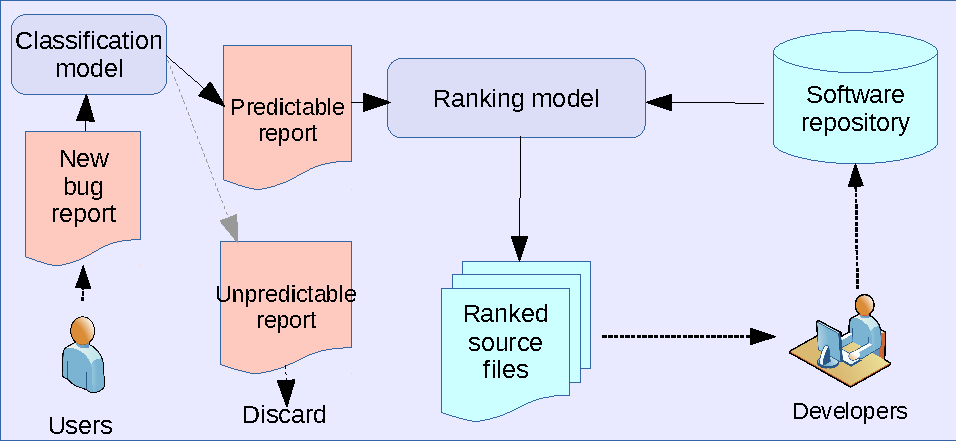
\includegraphics[width=\columnwidth]{figures/prefiltering.pdf}
\caption{High level architecture: pre-filtering before ranking.}
\label{fig:prefiltering architecture}
\end{figure}
Figure~\ref{fig:prefiltering architecture} shows the high level architecture of our bug report pre-filtering approach. When a new bug report is received, it will first be classified by a classification model into one of the two categories: ``predictable'' and ``unpredictable''. A ``predictable'' report is considered as informative and helpful to an IR-based ranking system for bug locating. It serves as input to the ranking system, which uses the report content to rank all the source code files and recommend the top ranked ones as ``buggy'' to developers to review. An ``unpredictable'' report, instead, is considered unhelpful to the IR-based ranking system and will be discarded. By keeping silent on unhelpful reports, the ranking system can reduce the number of false positives and make the recommendations be more trustworthy.

\section{LSTM-based Bug Report Classification}
\label{sec:lstm-based classification}
asdasdasdasdasdasdasdasdsdasda asd dasd asdasdasdasdasdasdasdasdsdasda asd dasd asdasdasdasdasdasdasdasdsdasda asd dasd asdasdasdasdasdasdasdasdsdasda asd dasd asdasdasdasdasdasdasdasdsdasda asd dasd asdasdasdasdasdasdasdasdsdasda asd dasd asdasdasdasdasdasdasdasdsdasda asd dasd asdasdasdasdasdasdasdasdsdasda asd dasd asdasdasdasdasdasdasdasdsdasda asd dasd asdasdasdasdasdasdasdasdsdasda asd dasd asdasdasdasdasdasdasdasdsdasda asd dasd asdasdasdasdasdasdasdasdsdasda asd dasd asdasdasdasdasdasdasdasdsdasda asd dasd asdasdasdasdasdasdasdasdsdasda asd dasd asdasdasdasdasdasdasdasdsdasda asd dasd asdasdasdasdasdasdasdasdsdasda asd dasd asdasdasdasdasdasdasdasdsdasda asd dasd asdasdasdasdasdasdasdasdsdasda asd dasd asdasdasdasdasdasdasdasdsdasda asd dasd asdasdasdasdasdasdasdasdsdasda asd dasd asdasdasdasdasdasdasdasdsdasda asd dasd asdasdasdasdasdasdasdasdsdasda asd dasd asdasdasdasdasdasdasdasdsdasda asd dasd asdasdasdasdasdasdasdasdsdasda asd dasd asdasdasdasdasdasdasdasdsdasda asd dasd asdasdasdasdasdasdasdasdsdasda asd dasd asdasdasdasdasdasdasdasdsdasda asd dasd asdasdasdasdasdasdasdasdsdasda asd dasd 
\begin{figure}[t]
\centering
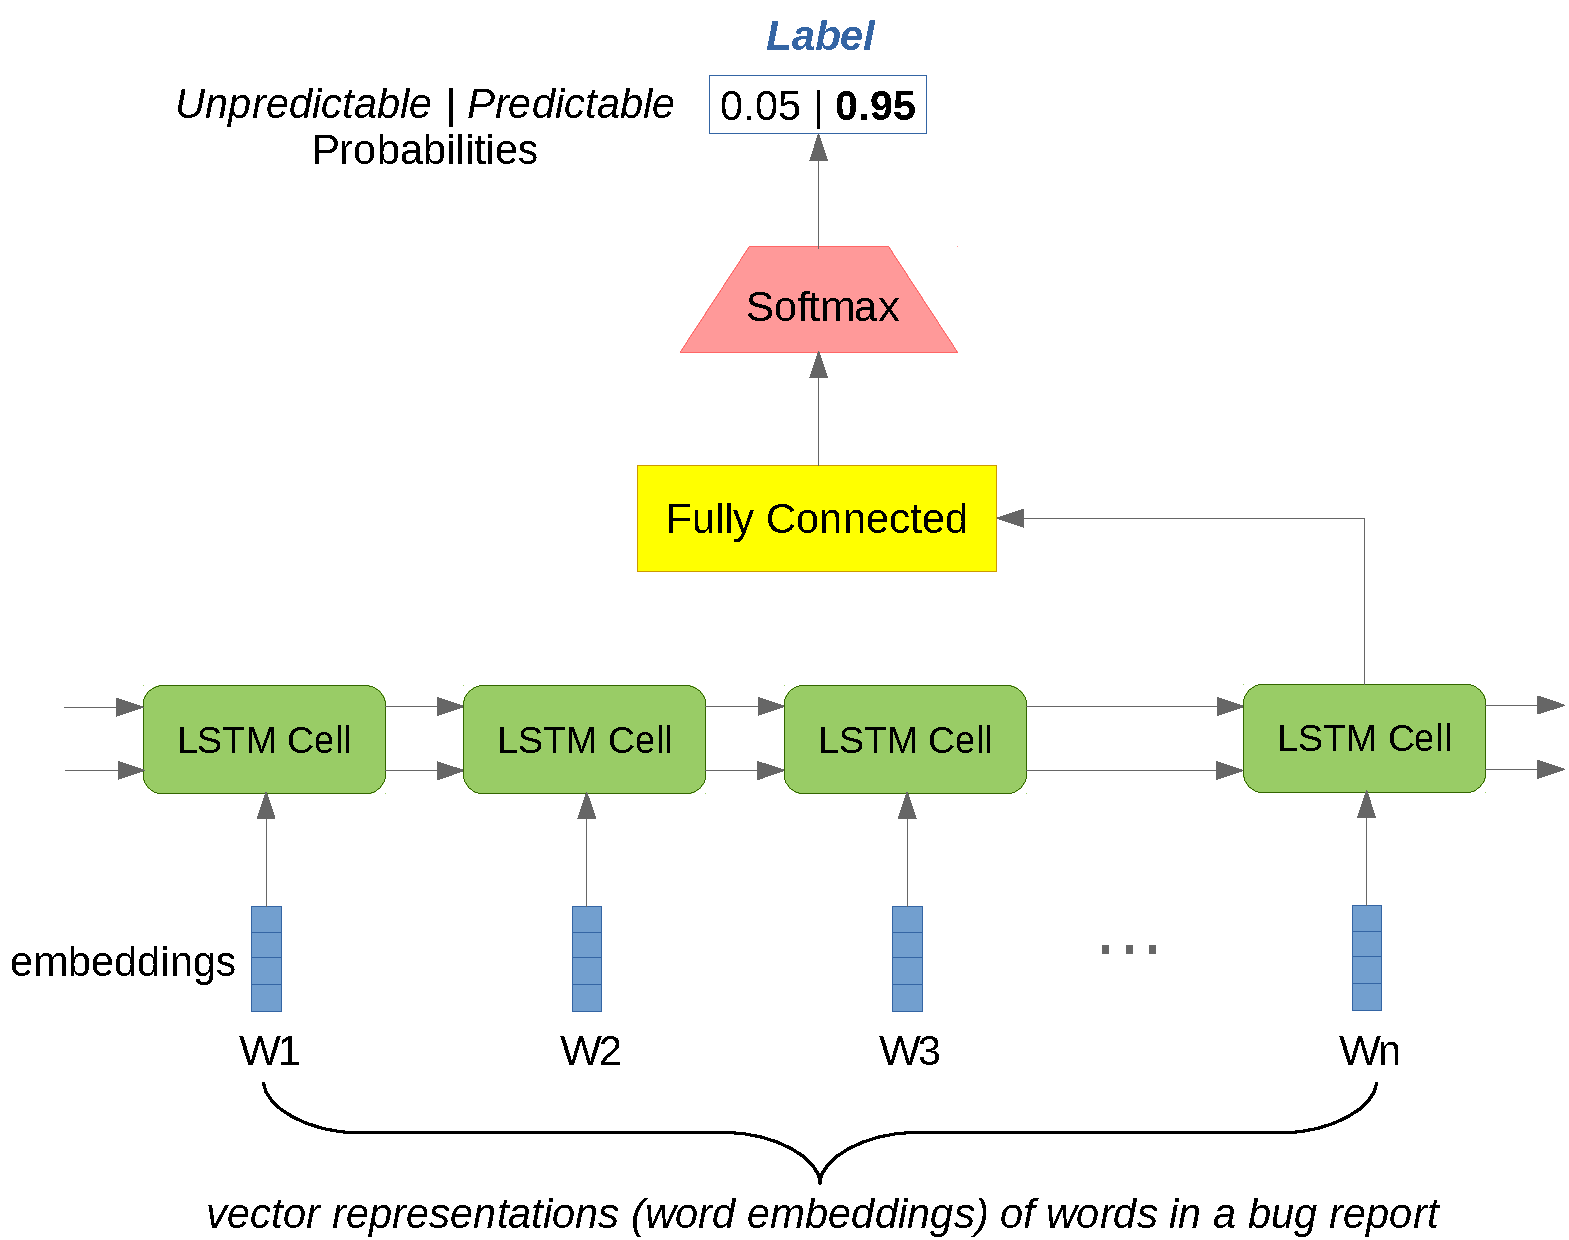
\includegraphics[width=\columnwidth]{figures/lstm.pdf}
\caption{Bug-report classification architecture: using LSTM.}
\label{fig:lstm}
\end{figure}

\begin{figure}[t]
\centering
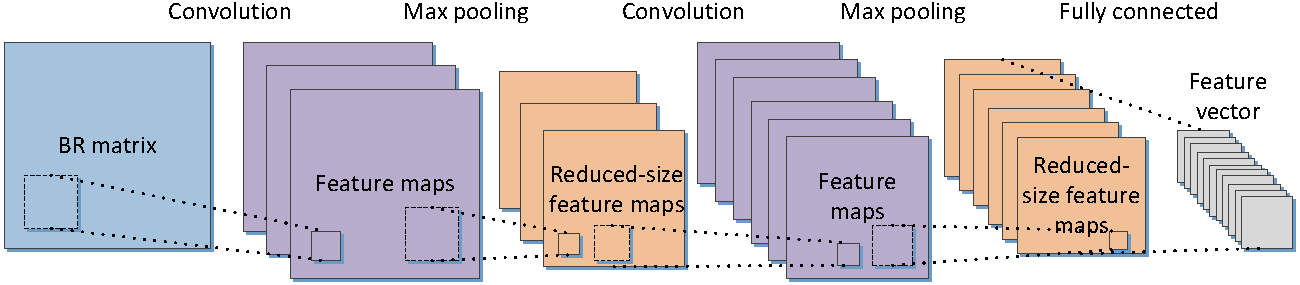
\includegraphics[width=\columnwidth]{figures/cnn.pdf}
\caption{Bug-report classification architecture: using CNN.}
\label{fig:cnn}
\end{figure}



\subsubsection{C.5 Evaluation}
We will evaluate the software defect positioning system on several large-scale open-source projects that contain a sufficient number (more than 2,000) of source code files and previously fixed bug reports. We will conduct experiments on software projects that are written in Java as well as projects written in C/C++ because these programming languages are widely used in both industry and academic. We will use projects from the Eclipse foundation~\footnote{https://eclipse.org/} and Apache foundation~\footnote{https://www.apache.org/} because 1) both have many large-scale open-source projects written in Java and C/C++; 2) the source code packages can be easily downloaded from their GIT repositories; 3) their bug reports or issue reports are public accessible. More specifically, the projects used in our preliminary work \cite{Ye:TSE15} will be used in this study. Additionally, we will run experiments on more projects such as Apache HTTP Server~\footnote{https://httpd.apache.org/} written in C, Lucene~\footnote{https://lucene.apache.org/} (an information retrieval software library) written in Java, and Hadoop~\footnote{http://hadoop.apache.org/} (a software framework for distributed storage and bigdata processing) written in Java. The selection of bug reports for evaluation is based on the same heuristics in \cite{Dallmeier:2007:EBL:1321631.1321702,Ye:FSE14}.

We will run the system to rank all the source code files for a given bug report and compare the result with the actual fix. The evaluation metrics such as \textit{Mean Average Precision} (MAP) \cite{Manning:2008:IIR:1394399} used in our preliminary work \cite{Ye:TSE15} will also be used in this study. Additionally, we will use Normalized Discounted Cumulative Gain (NDCG) \cite{Jarvelin:2002:CGE:582415.582418}, which is widely used in evaluating information retrieval models e.g. web search engines, to evaluate our system.

The PI is aware that user study is an effective way to evaluate the effectiveness of the proposed system in developers' real work. However, this is not the main goal of the proposed study. So the PI leave this to future work after the system is published. This study will also provide the basis for our future research on evaluating the effectiveness and usability of the proposed system in assisting teaching software engineering course at CSUSM.

\subsection{D. Work Plan}
The PI plan to hire one graduate student enrolled in the Master of Science Program in Computer Science (CS) and one undergraduate student enrolled in the Bachelor of Science in Computer Science program at CSUSM to help develop the system. The PI takes the overall responsibility of directing the project and keeps mentoring the students during the development.

\textbf{In the first year}, the graduate student will help implement the bug-report classification model, the LSTM-based semantic similarity feature, and the ranking model running on the server-side. The undergraduate student will implement the client-side programs and the web server that takes charge of the communication between the ranking model and the client-program. Since the ranking model, the database, and the web server work closely, the students will also work together closely during the development.

\textbf{In the second year}, two students will take charge of the maintenance and improvement of the system. Additionally, the graduate student will help run experiments to evaluate the ranking performance of the system on several open-source software projects, analyze the results, and improve the system accordingly. The undergraduate student will help develop a supplemental 3-D VR software visualization module. By the end of this year, the practical system will be published.

\textbf{Recruitment of students} will begin in spring, about three months before they start to work on the project. The PI will broadcast a hiring advertisement on CS-major electronic mailing lists, post a flier on class forums, and make a presentation of the project in the college-wide Frontiers in Science talk. In the coming 2017-2018 academic year, the CS department at CSUSM has a total of 866 undergraduate enrollments and a total of 39 graduate enrollments. Many students have desire to gain hands-on experience by working with faculty members on research projects. The PI will interview interested students. Preference will be given to economically-disadvantaged students, minority students, students making good progress toward their degree, and students who have demonstrated interest in this project.

\subsection{E. Broader Impacts}
The proposed study will result in a practical software system that alleviates develops' effort in bug finding and improves productivity. The system will be published. Any software developers can use and test it on their own projects. The system will be used in the software engineering courses at CSUSM to help students learn software engineering concepts in a lively manner. This project will expose students to an up-to-date software engineering research topic as well as some cutting-edge techniques including artificial neural networks and virtual reality.

The research outcome of this project will provide the basis for the PI's future research in performing user study and collecting user feedback to evaluate the effectiveness of the system in both academic and industry. The experience learned from this project will be very helpful for PI's research in code recommendation and automatic programming. The methodology and techniques used in this project will contribute to the software engineering research community.

The PI graduated with a Ph.D. degree from Ohio University at May 2016 and joined the CS department at CSUSM as an tenure-track faculty at August 2016. The funding to the proposed study will help the PI obtain important computing resources for building a software engineering (SE) research lab at CSUSM to continue his research. This fund, which supports two student assistants, will also help the PI found an SE research group at CSUSM. The research group will work on adapting new techniques to solve SE tasks, applying up-to-date SE research outcome to assist teaching SE courses, and engaging students in doing SE research projects.

The funding will have a significant impact on the quality of education for students here at CSUSM. The funds requested for student assistants will allow some of our economically-disadvantaged students, may of whom work in retail and on campus dining, to have paid positions during the academic year and summer.

Furthermore, funding of the proposed research program will create new opportunities for our students that have strong desire to participate in research projects. The research opportunities created from the funding of the proposed research will directly contribute to providing talented undergraduates at CSUSM with the research experience necessary to be competitive applicants for top-tier Ph.D. programs.

\begin{acks}
  The authors would like to thank Dr. Yuhua Li for providing the
  MATLAB code of the \textit{BEPS} method.

  The authors would also like to thank the anonymous referees for
  their valuable comments and helpful suggestions. The work is
  supported by the \grantsponsor{GS501100001809}{National Natural
    Science Foundation of
    China}{http://dx.doi.org/10.13039/501100001809} under Grant
  No.:~\grantnum{GS501100001809}{61273304}
  and~\grantnum[http://www.nnsf.cn/youngscientists]{GS501100001809}{Young
    Scientists' Support Program}.

\end{acks}

\section{Evaluation}
\label{sec:evaluation}

In this section, we describe an extensive set of experiments that are intended to determine the utility of the new document similarity measures based on word embeddings in the context of bug localization. This is an information retrieval task in which queries are bug reports and the system is trained to identify relevant, buggy files.

\begin{table*}[!thbp]
\centering
\caption{Benchmark Projects: {\it Eclipse$^*$ refers to Eclipse Platform UI.}}
\begin{tabular}{|c|c|c|c|c|c|c|} \hline
Project&Time Range&\# of bug reports&\# of bug reports&\# of bug reports&total\\
&&used for testing&used for training&used for tuning&\\ \hline
Birt&2005-06-14 -- 2013-12-19&583&500&1,500&2,583\\ \hline
Eclipse$^*$ &2001-10-10 -- 2014-01-17&1,656&500&1,500&3,656\\ \hline
JDT&2001-10-10 -- 2014-01-14&632&500&1,500&2,632\\ \hline
SWT&2002-02-19 -- 2014-01-17&817&500&1,500&2,817\\ \hline
\end{tabular}
\label{tab:dataset}
\end{table*}

\subsection{Text Pre-processing}
\label{sec:tokenization}

There are three types of text documents used in the experimental evaluations in this section: 1) the Eclipse API reference, developer guides, Java API reference, and Java tutorials that are used to train the word embeddings; 2) the bug reports; and 3) the source code files. When creating bag-of-words for these documents, we use the same pre-processing steps on all of them: we remove punctuation and numerical numbers, then split the text by whitespace. 

The tokenization however is done differently for each category of documents. In the one-vocabulary setting, compound words in the bug reports and the source code files are split based on capital letters. For example, ``WorkbenchWindow'' is split into ``Workbench'' and ``Window'', while its original form is also reserved. We then apply the Porter stemmer on all words/tokens.

In the two-vocabulary setting, a code token such as a method name ``{\it clear} is marked as ``@clear@'' so that it can be distinguished from the adjective ``clear''. Then we stem only the natural language words. We also split compound natural language words. In order to separate code tokens from natural language words in the training corpus, we wrote a dedicated HTML parser to recognize and mark the code tokens. For bug reports, we mark words that are not in an English dictionary as code tokens. For source code files, all tokens except those in the comments are marked as code tokens. Inside the comments, words that are not in an English dictionary are also marked as code tokens. 

\subsection{Corpus for Training Word Embeddings}
\label{sec:evaluation:training corpus}

To train the shared embeddings, we created a corpus from documents in the following Eclipse repositories: the Platform API Reference, the JDT API Reference, the Birt API Reference, the Java SE 7 API Reference, the Java tutorials, the Platform Plug-in Developer Guide, the Workbench User Guide, the Plug-in Development Environment Guide, and the JDT Plug-in Developer Guide. The number of documents and words/tokens in each repository are shown in Table~\ref{tab:corpus}. All documents are downloaded from their official website\footnote{\url{http://docs.oracle.com/javase/7/docs}}\footnote{\url{http://www.eclipse.org/documentation}}.  Code tokens in these documents are usually placed between special HTML tags such as $\langle${\it code}$\rangle$ or emphasized with different fonts.

\begin{table}[thbp]
\centering
\caption{Documents for training word embeddings.}
\begin{adjustbox}{width=0.47\textwidth}
\begin{tabular}{|c|c|c|} \hline
Data sources & Documents & Words/Tokens\\ \hline \hline
Platform API Reference & 3,731 & 1,406,768\\ \hline
JDT API Reference & 785 & 390,013\\ \hline
Birt API Reference & 1,428 & 405,910\\ \hline
Java SE 7 API Reference & 4,024 & 2,840,492\\ \hline
The Java Tutorials  & 1,282 & 1,024,358\\ \hline
Platform Plug-in Developer Guide & 343 & 182,831\\ \hline
Workbench User Guide & 426 & 120,734\\ \hline
Plug-in Development Environment Guide & 269 & 90,356\\ \hline
JDT Plug-in Developer Guide & 164 & 64,980\\ \hline
Total & 12,452 & 6,526,442\\ \hline
\end{tabular}
\end{adjustbox}
\label{tab:corpus}
\end{table}
\vspace*{-1em}
\begin{table}[ht!]
\centering
\caption{The vocabulary size.}
\begin{tabular}{|c|c|} \hline
Word embeddings trained on: & Vocabulary size\\ \hline
one-vocabulary setting & 21,848\\ \hline
two-vocabulary setting & 25,676\\ \hline
\end{tabular}
\label{tab:vocabulary}
\end{table}
\vspace*{-1em}
\begin{table}[ht!]
\centering
\caption{Number of word pairs.}
\begin{tabular}{|c|c|} \hline
Approach & \# of word pairs\\ \hline
One-vocabulary embeddings & 238,612,932\\ \hline
Two-vocabulary embeddings & 329,615,650\\ \hline
SEWordSim \cite{Tian:2014:SSW:2591062.2591071} & 5,636,534\\ \hline
SWordNet \cite{6224276} & 1,382,246\\ \hline
\end{tabular}
\label{tab:number of word pairs}
\end{table}

To learn the shared embeddings, we used the Skip-gram model, modified such that it works in the training scenarios described in Section~\ref{sec:embeddings2}. Table~\ref{tab:vocabulary} shows the number of words in each vocabulary setting.  Table~\ref{tab:number of word pairs} compares the number of word pairs used to train word embeddings in the one- and two-vocabulary settings with the number of word pairs used in two related approaches. Thus, when word embeddings are trained on the one-vocabulary setting, the vocabulary size is 21,848, which leads to 238,612,932 word pairs during training. This number is over 40 times the number of word pairs in SEWordSim \cite{Tian:2014:SSW:2591062.2591071}, and is more than 172 times the number of word pairs in SWordNet \cite{6224276}.

\subsection{Benchmark Datasets}
\label{sec:evaluation:subject systems}

We perform evaluations on the fined-grained benchmark dataset from \cite{Ye:FSE14}. Specifically, we use four open-source Java projects: Birt\footnote{\url{https://www.eclipse.org/birt/}}, Eclipse Platform UI\footnote{\url{http://projects.eclipse.org/projects/eclipse.platform.ui}}, JDT\footnote{\url{http://www.eclipse.org/jdt/}}, and SWT\footnote{\url{http://www.eclipse.org/swt/}}. For each of the 10,000 bug reports in this dataset, we {\it checkout} a before-fixed version of the source code, within which we rank all the source code files for the specific bug report.

Since the training corpus for word embeddings (shown in Table~\ref{tab:corpus}) contains only Java SE 7 documents, for testing we use only bug reports that were created for Eclipse versions starting with 3.8, which is when Eclipse started to add Java SE 7 support. The Birt, JDT, and SWT projects are all Eclipse Foundation projects, and also support Java SE 7 after the Eclipse 3.8 release. Overall, we collect for testing 583, 1656, 632, and 817 bug reports from Birt, Eclipse Platform UI, JDT, and SWT, respectively. Older bug reports that were reported for versions before release 3.8 are used for training and tuning the learning-to-rank systems.

Table~\ref{tab:dataset} shows the number of bug reports from each project used in the evaluation. The methodology used to collect the bug reports is discussed at length in \cite{Ye:FSE14}. Here we split the bug reports into a testing set, a training set, and a tuning set. Taking Eclipse Platform UI for example, the newest 1,656 bug reports, which were reported starting with Eclipse 3.8, are used for testing. The older 500 bug reports in the training set are used for learning the weight parameters of the ranking function in Equation~\ref{eq:file score}, using the SVM$^{rank}$ package \cite{Joachims:2002:OSE:775047.775067, Joachims:2006:TLS:1150402.1150429}. The oldest 1,500 bug reports are used for tuning the hyper-parameters of the Skip-gram model and the $SVM^{rank}$ model, by repeatedly training on 500 and testing on 1000 bug reports. To summarize, we tune the hyper-parameters of the Skip-gram model and the SVM$^{rank}$ model on the tuning dataset, then train the weight vector used in the ranking function on the training dataset, and finally test and report the ranking performance on the testing dataset. After tuning, the Skip-gram model was train to learn embeddings of size 100, with a context window of size 10, a minimal word count of 5, and a negative sampling of 25 words. 


\subsection{Results and Analysis}
\label{sec:evaluation:results and analysis}

We ran extensive experiments for the bug localization task, in order to answer the following research questions:
\begin{enumerate}
  \item[\textit{RQ1:}] Do word embeddings help improve the ranking performance, when added to an existing strong baseline?
  \item[\textit{RQ2:}] Do word embeddings trained on different corpora change the ranking performance?
  \item[\textit{RQ3:}] Do the word embedding training heuristics improve the ranking performance, when added to the vanilla Skip-gram model?
  \item[\textit{RQ4:}] Do the modified text similarity functions improve the ranking performance, when compared with the original similarity function in \cite{mihalcea:aaai06}?
\end{enumerate}

We use the Mean Average Precision (MAP) \cite{Manning:2008:IIR:1394399}, which is the mean of the average precision values for all queries, and the Mean Reciprocal Rank (MRR) \cite{Voorhees99thetrec-8}, which is the harmonic mean of ranks of the first relevant documents, as the evaluation metrics. MAP and MRR are standard evaluation metrics in IR, and were used previously in related work on bug localization \cite{Saha:2013:ASE:6693093, Ye:FSE14,Zhou:2012:BFM:2337223.2337226}.


\subsubsection{\textbf{RQ1:} Do word embeddings help improve the ranking performance?}
\label{sec:evaluation:rq1}

\begin{table}[t]
\centering
\caption{MAP and MRR for the 5 ranking systems.}
\begin{adjustbox}{width=0.47\textwidth}
\begin{tabular}{|c|c|c|c|c|c|c|} \hline
Project & Metric & LR+WE$^1$ & LR+WE$^2$ & LR & WE$^1$ & WE$^2$\\
& & $\phi_1$-$\phi_8$ & $\phi_1$-$\phi_8$ & $\phi_1$-$\phi_6$ & $\phi_7$-$\phi_8$ &$\phi_7$-$\phi_8$ \\ \hline
Eclipse & MAP & 0.40 & 0.40 & 0.37 & 0.26 & 0.26\\
Platform UI& MRR & 0.46 & 0.46 & 0.44 & 0.31 & 0.31\\ \hline
JDT& MAP & 0.42 & 0.42 & 0.35 & 0.22 & 0.23\\
& MRR & 0.51 & 0.52 & 0.43 & 0.27 & 0.29\\ \hline
SWT& MAP & 0.38 & 0.38 & 0.36 & 0.25 & 0.25\\
& MRR & 0.45 & 0.45 & 0.43 & 0.30 & 0.30\\ \hline
Birt& MAP & 0.21 & 0.21 & 0.19 & 0.13 & 0.13\\
& MRR & 0.27 & 0.27 & 0.24 & 0.17 & 0.17\\ \hline
\end{tabular}
\end{adjustbox}
\label{tab:comparison}
\end{table}

The results shown in Table~\ref{tab:comparison} compare the \textbf{LR} system introduced in  \cite{Ye:FSE14} with a number of systems that use word embeddings in the one- and two-vocabulary settings, as follows: \textbf{LR+WE$^1$} refers to combining the one-vocabulary word-embedding-based features with the six features of the LR system from \cite{Ye:FSE14}, \textbf{LR+WE$^2$} refers to combining the two-vocabulary word-embedding-based features with the LR system, \textbf{WE$^1$} refers to using only the one-vocabulary word-embedding-based features, and \textbf{WE$^2$} refers to using only the two-vocabulary word-embedding-based features. The parameter vector of each ranking system is learned automatically. The results show that the new word-embedding-based similarity features, when used as additional features, improve the performance of the \textbf{LR} system. The results of both \textbf{LR+WE$^1$} and \textbf{LR+WE$^2$} show that the new features help achieve 8.1\%, 20\%, 5.6\%, and 16.7\% relative improvements in terms of MAP over the original \textbf{LR} approach, for Eclipse Platform UI, JDT, SWT, and Birt respectively. In \cite{Ye:FSE14}, \textbf{LR} was reported to outperform other state-of-the-art bug localization models such as the VSM-based BugLocator from Zhou et al. \cite{Zhou:2012:BFM:2337223.2337226} and the LDA-based BugScout from Nguyen et al. \cite{Nguyen:2011:TAN:2190078.2190181}.

Another observation is that using word embeddings trained on one-vocabulary and using word embeddings trained on two-vocabulary achieve almost the same results.
% The advantage of using two-vocabulary is that natural language words such as the adjective \textit{clear} can be distinguished from the method name {\tt @clear@}, so the Skip-gram model would not use the context of the method name {\tt @clear@} to train the word embedding for the adjective \textit{clear}. But the results do not show a significant difference.
By looking at a sample of API documents and code, we discovered that class names, method names, and variable names are used with a consistent meaning throughout. For example, developers use \textit{Window} to name a class that is used to create a window instance, and use \textit{open} to name a method that performs an open action. Therefore, we believe the two-vocabulary setting will be more useful when word embeddings are trained on both software engineering (SE) and natural language (NL) corpora (e.g. Wikipedia), especially in situations in which a word has NL meanings that do not align well with its SE meanings. For example, since {\it eclipse} is used in NL mostly with the astronomical sense, it makes sense for {\it eclipse} to be semantically more similar with {\it light} than {\it ide}. However, in SE, we want {\it eclipse} to be more similar to {\it ide} and {\it platform} than to {\it total}, {\it color},  or {\it light}. By training separate embeddings for {\it eclipse} in NL contexts (i.e. {\it eclipse\_NL}) vs. {\it eclipse} in SE contexts (i.e. {\it eclipse\_SE}), the expectation is that, in an SE setting, the {\it eclipse\_SE} embedding would be more similar with the {\it ide\_SE} embedding than the {\it total\_SE} or {\it color\_SE} embeddings. 
% This would be especially useful when the word embeddings are trained on both SE text and Wikipedia text.
% Thus, although we distinguish {\tt @Window@} in code from \textit{window} in natural languages, their trained word embeddings are very similar. We believe this is the main reason why \textbf{LR+WE$^1$} and \textbf{LR+WE$^2$} achieve almost the same results. 

Kochhar et al. \cite{Kochhar:2014:PBB:2642937.2642997} reported from an empirical study that the localized bug reports, which explicitly mention the relevant file names, ``{\it statistically significantly and substantially}'' impact the bug localization results. They suggested that there is no need to run automatic bug localization techniques on these bug reports. Therefore, we separate the testing bug reports for each project into two subsets T1 (easy) and T2 (difficult). Bug reports in T1 mention either the relevant file names or their top-level public class names, whereas T2 contains the other bug reports. Note that, although bug reports in T1 make it easy for the programmer to find a relevant buggy file, there may be other relevant files associated with the same bug report that could be more difficult to identify, as shown in the statistics from Table~\ref{tab:comparison on T1 and T2}.

%\begin{table}[ht]
%\centering
%\caption{Number of bug reports that contain (T1) and do not contain (T2) the relevant file names.}
%\begin{tabular}{|c|c|c|c|} \hline
%Project & T1 & T2 & Total for testing \\ \hline
%Eclipse Platform UI& 322 & 1,334 & 1,656\\ \hline
%JDT & 84 & 548 & 632 \\ \hline
%SWT & 376 & 441 & 817 \\ \hline
%Birt & 27 & 556 & 583 \\ \hline
%\end{tabular}
%\label{tab:number of bug reports in T1 and T2}
%\end{table}

\begin{table}
\centering
\caption{Results on easy (T1) vs. difficult (T2) bug reports, together with \# of bug reports (size) and average \# of relevant files per bug report (avg).}
\begin{adjustbox}{width=0.47\textwidth}
\begin{tabular}{|c|c|cc|cc|} \cline{3-6}
\multicolumn{2}{c|}{} & \multicolumn{2}{c|}{T1} & \multicolumn{2}{c|}{T2} \\ \cline{3-6}
\multicolumn{2}{c|}{} & LR+WE$^1$ & LR & LR+WE$^1$ & LR \Tstrut\Bstrut\\ \hline
 & Size/Avg & \multicolumn{2}{c|}{322/2.11} & \multicolumn{2}{c|}{1,334/2.89} \\ \cline{2-6}
Eclipse & MAP & 0.80 & 0.78 & 0.30 & 0.27 \\
 & MRR & 0.89 & 0.87 & 0.36 & 0.33 \\ \hline
 & Size/Avg & \multicolumn{2}{c|}{84/2.60} & \multicolumn{2}{c|}{548/2.74} \\ \cline{2-6}
JDT & MAP & 0.79 & 0.75 & 0.36 & 0.29 \\
& MRR & 0.90 & 0.87 & 0.45 & 0.37 \\ \hline
 & Size/Avg & \multicolumn{2}{c|}{376/2.35} & \multicolumn{2}{c|}{441/2.57} \\ \cline{2-6} 
SWT & MAP & 0.57 & 0.55 & 0.22 & 0.21 \\
& MRR & 0.66 & 0.65 & 0.27 & 0.26 \\ \hline
 & Size/Avg & \multicolumn{2}{c|}{27/2.48} & \multicolumn{2}{c|}{556/2.24} \\ \cline{2-6}
Birt & MAP & 0.48 & 0.54 & 0.20 & 0.17 \\
& MRR & 0.62 & 0.69 & 0.25 & 0.22 \\ \hline
\end{tabular}
\end{adjustbox}
\label{tab:comparison on T1 and T2}
\end{table}

Table~\ref{tab:comparison on T1 and T2} shows the MAP and MRR results on T1 and T2. Because \textbf{LR+WE$^1$} and \textbf{LR+WE$^2$} are comparable on the test bug reports, here we compare only \textbf{LR+WE$^1$} with \textbf{LR}. The results show that both \textbf{LR+WE$^1$} and \textbf{LR} achieve much better performance on bug reports in T1 than T2 for all projects. This confirms the conclusions of the empirical study from Kochhar et al. \cite{Kochhar:2014:PBB:2642937.2642997}. 
% For bug reports in T1 that already mention the buggy file names, developers may easily locate the bug. However, the ranking system cannot achieve 100\% precision on these localized reports. So just as Kochhar et al. suggested \cite{Kochhar:2014:PBB:2642937.2642997}, we may not need to run automatic localization approaches for these bug reports.
The results in Table~\ref{tab:comparison on T1 and T2} also show that overall using word embeddings helps on both T1 and T2. One exception is Birt, where the use of word embeddings hurts performance on the 27 easy bugs in T1, a result that deserves further analysis in future work.

To summarize, we showed that using word embeddings to create additional semantic similarity features helps improve the ranking performance of a state-of-the-art approach to bug localization. However, separating the code tokens from the natural language words in two vocabularies when training word embeddings on the SE corpus did not improve the performance. In future work, we plan to investigate the utility of the two-vocabulary setting when training with both SE and NL corpora.


\subsubsection{\textbf{RQ2:} Do word embeddings trained on a different corpora change the ranking performance?}
\label{sec:evaluation:rq3}

To test the impact of the training corpus, we train word embeddings in the one-vocabulary setting using the Wiki data dumps\footnote{\url{https://dumps.wikimedia.org/enwiki/}}, and redo the ranking experiment.
% I compare the results of this new experiment with the results shown in Table~\ref{tab:comparison}.
\begin{table}[thbp]
\centering
\caption{The size of the different corpora.}
\begin{tabular}{|c|c|c|} \hline
Corpus & Vocabulary & Words/Tokens\\ \hline \hline
Eclipse and Java & 21,848 & 6,526,442\\ \hline
% documents & & \\ \hline
Wiki & 2,098,556 & 3,581,771,341\\ \hline
\end{tabular}
\label{tab:different corpora}
\end{table}
%\vspace*{-1em}
\begin{table}[thbp]
\centering
\caption{Comparison of the \textbf{LR+WE$^1$} results when using word embeddings trained on different corpora.}
\begin{adjustbox}{width=0.47\textwidth}
\begin{tabular}{|c|c|c|c|c|c|} \hline
Corpus & Metric & Eclipse & JDT & SWT & Birt \\
& Metric & Platform UI & & & \\ \hline
Eclipse and Java & MAP & 0.40 & 0.42 & 0.38 & 0.21 \\
documents& MRR & 0.46 & 0.51 & 0.45 & 0.27 \\ \hline
Wiki & MAP & 0.40 & 0.41 & 0.38 & 0.21 \\
& MRR & 0.46 & 0.51 & 0.45 & 0.27 \\ \hline
\end{tabular}
\end{adjustbox}
\label{tab:comparison on different copora}
\end{table}
The advantage of using the Wiki corpus is its large size for training.
Table~\ref{tab:different corpora} shows the size of the Wiki corpus. The number of words/tokens in the Wiki corpus is 548 times the number in our corpus, while its vocabulary size is 96 times the vocabulary size of our corpus. Theoretically, the larger the size of the training corpus the better the word embeddings. On the other hand, the advantage of the smaller training corpus in Table~\ref{tab:corpus} is that its vocabulary is close to the vocabulary used in the queries (bug reports) and the documents (source code files).

Table~\ref{tab:comparison on different copora} shows the ranking performance by using the Wiki embeddings. Results show that the project specific embeddings achieve almost the same MAP and MRR for all projects as the Wiki embeddings. We believe one reason for the good performance of the Wiki embeddings is the pre-processing decision to split compound words such as {\tt WorkbenchWindow} that do not appear in the Wiki vocabulary into their components words {\tt Workbench} and {\tt Window}, which belong to the Wiki vocabulary. Correspondingly, Table~\ref{tab:wiki-vs-eclipse} below shows the results of evaluating just the word-embeddings features ({\bf WE}$^1$) on the Eclipse project with the two types of embeddings, with and without splitting compound words. As expected, the project-specific embeddings have better performance than the Wiki-trained embeddings when compound words are not split; the comparison is reversed when splitting is used.
\begin{table}[h]
\centering
\caption{Project-specific vs. Wikipedia embeddings performance of WE$^1$ features, with and without splitting compound words.}
%\begin{adjustbox}{width=0.47\textwidth}
\begin{tabular}{|c|c|c|c|} \hline
Project & Metric & No Split & Split \\ \hline
Eclipse/Java& MAP & 0.254 & 0.260 \\
 & MRR & 0.307 & 0.310 \\ \hline
Wikipedia & MAP & 0.248 & 0.288 \\
& MRR & 0.300 & 0.346 \\ \hline
\end{tabular}
%\end{adjustbox}
\label{tab:wiki-vs-eclipse}
\end{table}
Overall, each corpus has its own advantages: while the embeddings trained on the project-specific corpus may better capture specific SE meanings, the embeddings trained on Wikipedia may benefit from the substantially larger amount of training examples. Given the complementary advantages, in future work we plan to investigate training strategies that exploit both types of corpora.

%\begin{table}[htbp]
%\centering
%\caption{The vocabulary overlap between word embeddings trained on different corpora.}
%\begin{adjustbox}{width=0.47\textwidth}
%\begin{tabular}{|c|c|c|c|c|} \hline
% & Code & Reports & Java and Eclipse & Wiki \\ \hline
% Code & 51,747 & 7,368 & 8,174 & 7,960 \\ \hline
% Reports & 7,368 & 11,167 & 4,492 & 4,374 \\ \hline
% Java and Eclipse & 8,174 & 4,492 & 21,848 & 6,935 \\ \hline
% Wiki & 7,960 & 4,374 & 6,935 & 1,811,253\\ \hline
%\end{tabular}
%\end{adjustbox}
%\label{tab:corpus overlap}
%\end{table}
%Table~\ref{tab:corpus overlap} shows the overlap between the vocabularies of word embeddings trained on different corpora. The vocabulary of the Wiki embeddings in Table~\ref{tab:corpus overlap} is smaller than the vocabulary of the Wiki corpus in Table~\ref{tab:different corpora} because we perform stemming. In Table~\ref{tab:corpus overlap}, ``Code'' contains all the source code files of the Eclipse Platform UI project checkout at {\it commit 5da5952}, which is the before-fix version of the newest bug report in our benchmark dataset, ``Reports'' contains all the Eclipse Platform UI bug reports in our dataset, ``Java and Eclipse documents'' refers to the training corpus shown in Table~\ref{tab:corpus}, and ``Wiki'' refers to the Wiki corpus. As we can see from Table~\ref{tab:corpus overlap}, the vocabulary overlap between ``Code'' and ``Wiki'' is close to the vocabulary overlap between ``Code'' and ``Java and Eclipse Documents''. Similarly, the vocabulary overlap between ``Reports'' and ``Wiki'' is also close to the vocabulary overlap between ``Reports'' and ``Java and Eclipse Documents''. Although the Wiki corpus is huge, the vocabulary of bug reports and the source code files is small. Thus, the large size of the Wiki corpus does not translate into improved performance on the bug localization task. % Therefore, using a small corpus that contains Java and Eclipse project documents can achieve the same results with using the Wiki corpus. 


\subsubsection{\textbf{RQ3:} Do the word embedding training heuristics improve the ranking performance?}
\label{sec:evaluation:rq4}

Table~\ref{tab:comparison of skip-gram} shows the results of using the original Skip-gram model without applying the heuristic techniques discussed in Sections~\ref{sec:mapping1} and~\ref{sec:mapping2}. It shows that both the enhanced and the original Skip-gram model achieve the same results most of the time. These results appear to indicate that increasing the number of training pairs for word embeddings will not lead to further improvements in ranking performance, which is compatible with the results of using the Wiki corpus vs. the much smaller project-specific corpora.
\begin{table}[t]
\centering
\caption{\textbf{LR+WE$^1$} results obtained using the enhanced vs. the original Skip-gram model.}
\begin{adjustbox}{width=0.47\textwidth}
\begin{tabular}{|c|c|c|c|c|c|c|} \hline
Project & Metric & LR & Enhanced Skip-gram & Original Skip-gram\\
& & $\phi_1$-$\phi_8$ & $\phi_1$-$\phi_6$ & $\phi_1$-$\phi_8$ \\ \hline
Eclipse & MAP & 0.37 & 0.40 & 0.40 \\
Platform UI& MRR & 0.44 & 0.46 & 0.46 \\ \hline
JDT& MAP & 0.35 & 0.42 & 0.42 \\
& MRR & 0.43 & 0.51 & 0.51 \\ \hline
SWT& MAP & 0.36 & 0.38 & 0.37 \\
& MRR & 0.43 & 0.45 & 0.44 \\ \hline
Birt& MAP & 0.19 & 0.21 & 0.21 \\
& MRR & 0.24 & 0.27 & 0.27 \\ \hline
\end{tabular}
\end{adjustbox}
\label{tab:comparison of skip-gram}
\end{table}

\subsubsection{\textbf{RQ4:} Do the modified text similarity functions improve the ranking performance?}
\label{sec:evaluation:rq5}

Table~\ref{tab:comparison of text similarity function} below compares the new text similarity functions shown in Equation~\ref{eq:new tssim} with the original text similarity function from Mihalcea et al. \cite{mihalcea:aaai06}, shown in Equation~\ref{eq:tssim}. In \textbf{WE$^1_{ori}$}, the new features $\phi_7$ and $\phi_8$ are calculated using the one-vocabulary word embeddings and the original $idf$-weighted text similarity function. The results of \textbf{LR+WE$^1$} and \textbf{LR} are copied from Table~\ref{tab:comparison}, for which $\phi_7$ and $\phi_8$ are calculated using the new text similarity functions.

\begin{table}[ht]
\centering
\caption{Comparison between the new text similarity function (LR+WE$^1$) and the original similarity function (LR+WE$^1_{ori}$).}
\begin{adjustbox}{width=0.47\textwidth}
\begin{tabular}{|c|c|c|c|c|c|c|} \hline
Project & Metric & LR & LR+WE$^1$ & LR+WE$^1_{ori}$ \\
& & $\phi_1$-$\phi_8$ & $\phi_1$-$\phi_6$ & $\phi_7$-$\phi_8$ \\ \hline
Eclipse & MAP & 0.37 & 0.40 & 0.37\\
Platform UI& MRR & 0.44 & 0.46 & 0.43\\ \hline
JDT& MAP & 0.35 & 0.42 & 0.36\\
& MRR & 0.43 & 0.51 & 0.45\\ \hline
SWT& MAP & 0.36 & 0.38 & 0.37\\
& MRR & 0.43 & 0.45 & 0.44\\ \hline
Birt& MAP & 0.19 & 0.21 & 0.20\\
& MRR & 0.24 & 0.27 & 0.25\\ \hline
\end{tabular}
\end{adjustbox}
\label{tab:comparison of text similarity function}
\end{table}

Results show that the new text similarity features lead to better performance than using the original text similarity function. The new features obtain a 20\% relative improvement in terms of MAP over the \textbf{LR} approach, while features calculated based on the original text similarity function achieve only a 3\% relative improvement.

% The new text similarity function has a big impact on the system performance. The reasons of the superior of the new text similarity function over the original function on bug localization are discussed in Section~\ref{sec:text-to-code}.

\section{Evaluation of Word Embeddings for API Recommendation}
\label{sec:evaluation:SO}

% The last part of this section details a preliminary experiment using data collected from Stack Overflow for the API linking task (Section~\ref{sec:evaluation:SO}).
% An API linking task, in which queries are questions posted on Stack Overflow\footnote{http://stackoverflow.com}, and the system is supposed to identify API documents that may help the user in formulating the answer

To assess the generality of using document similarities based on word embeddings for information retrieval in software engineering, we evaluate the new similarity functions on the problem of linking API documents to Java questions posted on the community question answering (cQA) website Stack Overflow (SO). The SO website enables users to ask and answer computer programming questions, and also to vote on the quality of questions and answers posted on the website. In the Question-to-API (Q2API) linking task, the aim is to build a system that takes as input a user's question in order to identify API documents that have a non-trivial semantic overlap with the (as yet unknown) correct answer. We see such a system as being especially useful when users ask new questions, for which they would have to wait until other users post their answers. Recommending relevant API documents to the user may help the user find the answer on their own, possibly even before the correct answer is posted on the website. To the best of our knowledge, the Q2API task for cQA websites has not been addressed before.

In order to create a benchmark dataset, we first extracted all questions that were tagged with the keyword 'java', using the datadump archive available on the Stack Exchange website. Of the 1,493,883 extracted questions, we used a script to automatically select only the questions satisfying the following criteria:
\begin{enumerate}
	\item The question score is larger than 20, which means that more than 20 people have voted this question as ``useful''.
	\item The question has answers of which one was checked as the ``correct'' answer by the user who asked the question.
	\item The ``correct'' answer has a score that is larger than 10, which means that more than 10 people gave a positive vote to this answer.
	\item The ``correct'' answer contains at least one link to an API document in the official Java SE API online reference (versions 6 or 7).
\end{enumerate}
This resulted in a set of high quality 604 questions, whose correct answers contain links to Java API documents. We randomly selected 150 questions and asked two proficient Java programmers to label the corresponding API links as {\it helpful} or {\it not helpful}. The remaining 454 questions were used as a (noisy) training dataset. Out of the 150 randomly sampled questions, the 111 questions that were labeled by both annotators as having {\it helpful} API links were used for testing. The two annotators were allowed to look at the correct answer in order to determine the semantic overlap with the API document.

Although we allow API links to both versions 6 and 7, we train the word embeddings in the one-vocabulary setting, using only the Java SE 7 API documentations and tutorials. There are 5,306 documents in total, containing 3,864,850 word tokens. 

We use the Vector Space Model (VSM) as the baseline ranking system. Given a question $T$, for each API document $S$ we calculate the VSM similarity as feature $\phi_1(T, S)$ and the asymmetric semantic similarities that are based on word embeddings as features $\phi_2(T, S)$ and $\phi_3(T, S)$. In the VSM+WE system, the file score of each API document is calculated as the weighted sum of these three features, as shown in Equation~\ref{eq:file score}. During training on the 454 questions, the objective of the learning-to-rank system is to find weights such that, for each training question, the relevant (helpful) API documents are ranked at the top. During evaluation on the 111 questions in the test dataset, we rank all the Java API documents $S$ for each question $T$ in descending order of their ranking score $f(T, S)$.

\begin{table}[ht]
\centering
\caption{Results on the Q2API task.}
%\begin{adjustbox}{width=0.47\textwidth}
\begin{tabular}{|c|c|c|} \hline
Approach & MAP & MRR\\ \hline
VSM & 0.11 & 0.12\\ \hline
VSM+WE & 0.35 & 0.39 \\ \hline 
\end{tabular}
%\end{adjustbox}
\label{tab:comparison on SO questions}
\end{table}

Table~\ref{tab:comparison on SO questions} shows the MAP and MRR performance of the baseline VSM system that uses only the VSM similarity feature, vs. the performance of the VSM+WE system that also uses the two semantic similarity features. The results in this table indicate that the document similarity features based on word embeddings lead to substantial improvements in performance. As such, these results can serve as an additional empirical validation of the utility of word embeddings for information retrieval tasks in software engineering.

We note that these results are by no means the best results that we expect for this task, especially since the new features were added to a rather simple VSM baseline. For example, instead of treating SO questions only as bags of undifferentiated words, the questions could additionally be parsed in order to identify code tokens or code-like words that are then disambiguated and mapped to the corresponding API entities \cite{Bacchelli:2010:LES:1806799.1806855, Dagenais:2012:RTL:2337223.2337230, Subramanian:2014:LAD:2568225.2568313}. Given that, like VSM, these techniques are highly lexicalized, we expect their performance to improve if used in combination with additional features based on word embeddings. 

\section{Related Work}
\label{sec:related word}

In this section, we describe work in other areas of IR-based bug report handling, other uses of neural networks in software engineering, and briefly touch on non-IR-based approaches to bug report handling.

\subsection{Bug Report Handling}

Lam et al. \cite{7372035} seeks to improve bug report handling by automating the task of associating buggy files with a bug report.  In order to overcome the lexical mismatch problem of the natural language used in bug reports not matching the terms and code tokens in source files, they combined rSVM information retrieval with deep neural networks to associate terms in bug reports to terms in source files.  Their resulting model, DnnLoc, is able to suggest likely source code files that contain the bug described in a bug report.

Huo et al. \cite{Huo:2017:EUF:3172077.3172153, Huo:2016:LUF:3060832.3060845} propose a couple of approaches to localize buggy source files from a bug report.  They first propose a novel convolutional neural network NP-CNN that leverages the structural information of source code in addition to the lexical information to accomplish this task.  They follow with another model LS-CNN that combines CNN and LSTM to additionally utilize the sequential information of source code.

Ye et al. \cite{Ye:ICSE16, Ye:FSE14} develops a learning-to-rank model to combine various features for ranking source files for bug reports.  The model is trained using source code contents, API descriptions of the code, bug-fixing history, and the code change history information of previously solved bug reports.  Further work to bridge the lexical gap between bug reports and source files was done using word embeddings to train a model to estimate semantic similarities between bug reports, source code, and API/reference documents.

Zhou et al. \cite{Zhou:2012:BFM:2337223.2337226} implemented BugLocator that locates files based on ranking by textual similarity of bug reports and source code using a revised Vector Space Model (rSVM).  Sahar et al. \cite{Saha:2013:ASE:6693093} outperforms BugLocator with BLUiR that uses structural information of code to enable more accurate bug localization.

Kim et al. \cite{Kim:2013:WFT:2554428.2554437} apply Na\"{i}ve Bayes to localize source code files for a bug report based on previously fixed files as labels.  In order to improve localization accuracy, they add an initial phase where bug reports are classified to predictable or deficient based on prediction history of resolved bug reports.  Deficient bug reports are not localized to code to avoid misleading recommendations.

Lukins et al. \cite{Lukins:2010:BLU:1824820.1824850} use a Latent Dirichlet Allocation (LDA) based technique that is accurate and scaleable for automatic bug localization.  Nguyen et al. \cite{Nguyen:2011:TAN:2190078.2190181} uses the shared technical aspects in the text of bug reports and corresponding source code to implement a LDA based system BugScout to correlate reports to buggy code.

Rao et al. \cite{Rao:2011:RSL:1985441.1985451} compared Unigram Model, Vector Space Model, Latent Semantic Analysis Model, Latent Dirichlet Allocation Model, and Cluster Based Document Model for bug localization.  They found that more sophisticated models (LDA, LSA, CBDM) did not outperform simpler text models (UM, VSM).

Determining the severity of bug reports automatically is another area where handling of bug reports can be improved.  Lamkanfi et at. \cite{5463284} use a Na\"{i}ve Bayes based approach to investigate if severity can be accurately predicted.  They conclude that a sufficient training set can achieve reasonable prediction accuracy.  Zhang et al. \cite{Zhang:2016:TMA:2949080.2949249} describe a system to find similar historical bug reports utilizing a modified REP algorithm and K-Nearest Neighbor.  Then, an improved performance severity predicition algorithm is developed with the extracted features of the bug reports.

Another direction for reducing effort of handling bug reports is to automate triage of bug reports to developer(s) that are likely to resolve them.  Anvik et al. \cite{Anvik:2006:FTB:1134285.1134336, Anvik2011ReducingTE} used support vector machines and other machine learning approaches to implement developer recommending models achieving varying degrees of precision.  Hu et al. \cite{Hu2014EffectiveBT} implement recommendation method called Bug Fixer that utilizes historic information of source code components where developers have have fixed bugs previously.  Zhang et al. \cite{Zhang2013AHB} implement a hybrid system that utilizes unigram model to find similar bug reports and then recommends a developer based on developer's probability to fix and a model of developer's activity and experience.  Bhattacharya et al. \cite{Bhattacharya:2012:AHB:2330373.2330434} employ a set of machine learning tools and tossing graphs to accurately assign bugs to developers.  Xuan et al. \cite{Xuan2015TowardsEB} use a model of instance selection and feature selection determined by historic bug data sets to reduce data scale and improve accuracy of bug triage. Shokripour et al. \cite{Shokripour:2013:WSC:2487085.2487089} uses an approach that uses noun extraction and simple term weighting to predict bug location and then uses a location-based approach to recommend assigment of the bug to a developer.

\subsection{Using Neural Networks to Support Software Engineering}

Effort estimation is necessary for planning and managing a software project.  Choetkiertikul et al. \cite{8255666} utilizes deep learning with long short-term memory and recurrent highway network to facilitate effort estimation for agile projects.  They use deep learning to model and predict estimations of story points, a unit of measure for the effort to complete a user story or resolve an issue.

Developers often need to utilize APIs to implement functionality, but it can be a significant obstacle to deal with unfamiliar libraries or frameworks.  Gu et al. \cite{Gu:2016:DAL:2950290.2950334} utilize RNN Encoder-Decoder for a deep learning approach called DeepAPI.  DeepAPI allows a natural language query to accurately generate a relevant API sequence.

Online developer forums are full of individual units of programmer knowledge that have potential to be linked for being related, duplicates, etc.  Xu et al. \cite{Xu:2016:PSL:2970276.2970357} utilize word embeddings and convolutional neural networks for a deep learning based approach to semantically linking knowledge units on StackOverflow that outperforms traditional methods.  Fu et al. \cite{Fu:2017:EOH:3106237.3106256,} follow up this approach with a differential evolution approach that achieve similar results on the scale of minutes rather than hours with the deep learning approach.  They show that deep learning may provide benefits for software engineering but simpler or faster methods should still be considered.

\subsection{Non-IR-Based Bug Report Handling}

Information retrieval approaches are not the only way to try handling bug reports.  There are approaches that are not IR-based or augment/combine with IR to accomplish bug report handling tasks.  Cleve et al. \cite{Cleve:2005:LCP:1062455.1062522} focus on cause transitions to find locations of defects.  Dit et al. \cite{Dit:2013:IIR:2436118.2436134} utilizes web mining algorithms to analyze execution information.  Poshyvanyk et al. \cite{Poshyvanyk:2013:CLU:2377656.2377660, Poshyvanyk:2007:FLU:1263152.1263534} have utilized both Formal Concept Analysis and scenario-based probabilistic ranking of events.  Liu et al. \cite{Liu:2005:SSM:1081706.1081753} uses a model based on pattern evaluation between correct and incorrect runs to quantify bug-relevance.  Jin et al. \cite{Jin:2013:FFL:2483760.2483763} used synthesized passing and failing executions to perform fault localization.  Le et al \cite{Le:2015:IRS:2786805.2786880, B.Le:2016:LBF:2931037.2931049} utilizes approaches of program spectra analysis to find suspicious words and invariant mining.  Jones et al. \cite{Jones:2005:EET:1101908.1101949} implements Tarantula approach of generating likelihood/suspicion for each statement of source code using the code entities executed by passing and failing test cases.



\section{Future Work}
This is the future-work section.


\section{Conclusion}
This is the conclusion section.


\begin{acks}
  The authors would like to thank Dr. Yuhua Li for providing the
  MATLAB code of the \textit{BEPS} method.

  The authors would also like to thank the anonymous reviewers for
  their valuable comments and helpful suggestions.
\end{acks}


\bibliographystyle{ACM-Reference-Format}
\bibliography{bibliography}

\end{document}
